\documentclass[a4paper, 12pt]{article}%тип документа

%отступы
\usepackage[left=2cm,right=2cm,top=2cm,bottom=3cm,bindingoffset=0cm]{geometry}

%Русский язык
\usepackage[T2A]{fontenc} %кодировка
\usepackage[utf8]{inputenc} %кодировка исходного кода
\usepackage[english,russian]{babel} %локализация и переносы

%Вставка картинок
\usepackage{wrapfig}
\usepackage{graphicx}
\graphicspath{{pictures/}}
\DeclareGraphicsExtensions{.pdf,.png,.jpg}

%оглавление
\usepackage{titlesec}
\titlespacing{\chapter}{0pt}{-30pt}{12pt}
\titlespacing{\section}{\parindent}{5mm}{5mm}
\titlespacing{\subsection}{\parindent}{5mm}{5mm}
\usepackage{setspace}

%Графики
\usepackage{multirow}
\usepackage{pgfplots}
\pgfplotsset{compat=1.9}

%Математика
\usepackage{amsmath, amsfonts, amssymb, amsthm, mathtools}

%Заголовок
\author{Валеев Рауф Раушанович \\
группа 825}
\title{\textbf{Работа 3.5.3$^2$\\Релаксационные колебания }}
\newtheorem{task}{Задача}
\begin{document}
\maketitle
\newpage
\section*{Цель работы}
Изучение вольт-амперной характеристики нормального тлеющего разряда; исследование релаксационных колебаний генератора на стабилитроне.
\section*{В работе используются}
Стабилитрон на монтажной плате, магазин ёмкостей, магазин сопротивлений, источник питания, амперметр, вольтметр, осциллограф.
\section*{Описание установки}
\begin{wrapfigure}{l}{0.6\textwidth}
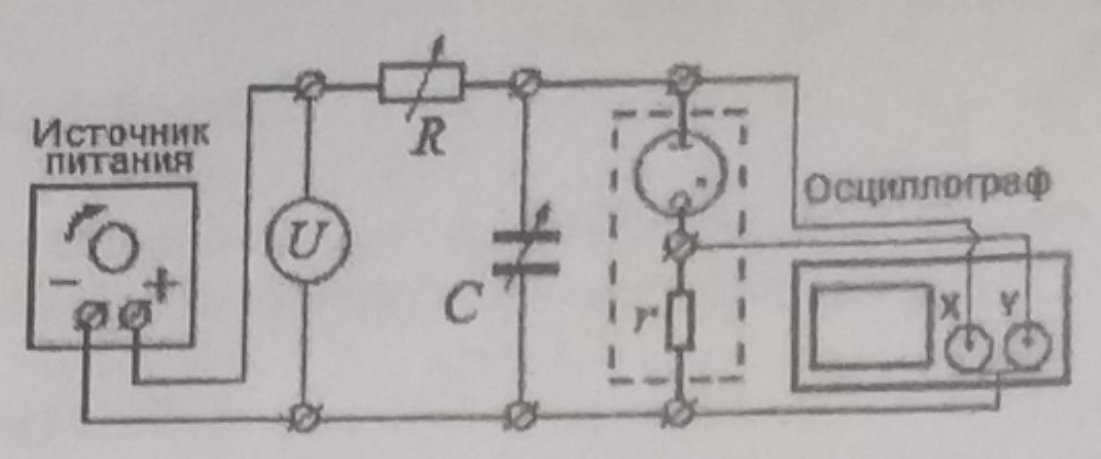
\includegraphics[width = 0.5\textwidth]{3.png}
\caption{Схема экспериментального стенда}
\end{wrapfigure}
Схема установке представлена на рис.1. Штриховой линией выделена панель, на которой установлен стабилитрон и последовательно с ним - сопротивление $r$, позволяющее предохранить диод от перегорания, а так же получить напряжение, пропорциональное току разряда, это сопротивление остается включенным при всех измерениях.

\section*{Теория}
\begin{wrapfigure}{l}{0.4\textwidth}
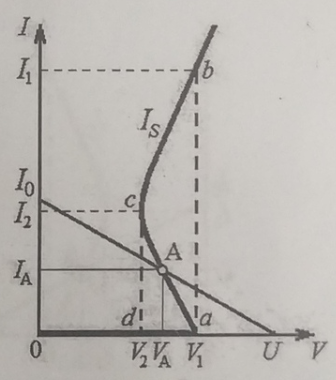
\includegraphics[width = 0.3\textwidth]{2.png}
\caption{Упрощенная вольт-амперная характеристика стабилитрона}
\end{wrapfigure}

В работе исследуются релаксационные колебания, возбуждаемые в электрическом контуре состоящем из ёмкости $C$, резистора $R$ и газоразрядного диода с $S$-образной вольт-амперной характеристикой. 

В данном случае сами колебания являются совокупностью двух апериодических процессов --- зарядки и разрядки конденсатора. 

Выясним, при каком условии возможен колебательный процесс. В стационарном режиме, когда напряжение $V$ на конденсаторе постоянно и $dV/dt = 0$, ток через лампу
\begin{equation}
I_{\text{ст}} = \dfrac{U - V}{R+r}
\end{equation}

Данное равенство представлено на рис. 2.

Рассмотрим, как происходит колебательный процесс, отсчитывая время с того момента, когда напряжение на конденсаторе $C$ равно $V_2$. При зарядке конденсатора через сопротивление $R$ напряжение на нём увеличивается (рис.3). Как только оно достигает напряжения зажигания $V_1$, лампа начнет проводить ток, причем прохождения тока сопровождается разрядкой конденсатора. 

\begin{figure}[h]
\begin{center}
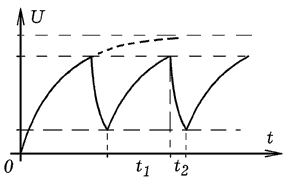
\includegraphics[width = 0.5\textwidth]{4.png}
\caption{Осциллограмма релаксационных колебаний}
\end{center}
\end{figure}

Рассчитаем период колебаний. Полное время одного периода колебаний --- $T$ состоит из суммы времени зарядки $\tau_{\text{з}}$ и времени разрядки $\tau_{\text{р}}$, но если сопротивление $R$ существенно превосходит сопротивление зажженной лампы и резистора $r$, то $\tau_{\text{з}} \gg \tau_{\text{р}}$ и $T \approx \tau_{\text{з}}$, что подтверждается в эксперименте. Во время зарядки конденсатора лампа не горит ($I(V) = 0$), и уравнение уравнение для напряжения принимает вид $V(t)$:
\begin{equation}
RC\dfrac{dV}{dt} = U-V
\end{equation}
Мы рассчитываем время с момента гашения лампы, поэтому $V = V_2$ при $t=0$.

Решим уравнение $(3)$ и получим, что 
\begin{equation}
V = U - (U - V_2) e^{-t/RC}
\end{equation}

В момент зажигания $V = V_1$, поэтому 
\begin{equation}
V_1 = U - (U - V_2) e^{-\tau_{\text{з}}/RC}
\end{equation}

Из уравнения $(4)$ получим, что 
\begin{equation}
T \approx \tau_{\text{з}} = \ln \dfrac{U - V_2}{U - V_1}
\end{equation}
\section*{Ход работы}
\subsection*{Характеристика стабилитрона}
Снимем часть вольт-амперной характеристики стабилитрона с сопротивлением $r = 5,1$ кОм. Снимем с возрастанием и с убыванием напряжения. В этой работе используются вольтметр с $\sigma_V = 0,2$ В и амперметр с $\sigma_I = 0,02$ мА. Представим эти данные в виде графиков.

\begin{table}[ht]
\begin{center}
\begin{tabular}{|c|c|c|ccc}
\hline
\multicolumn{3}{|c|}{возрастание $V$} & \multicolumn{3}{c|}{убывание $V$}                                                                    \\ \hline
$V$, В & $I$, мА & $V - r \cdot I$, В & \multicolumn{1}{c|}{$V$, В} & \multicolumn{1}{c|}{$I$, мА} & \multicolumn{1}{c|}{$V - r \cdot I$, В} \\ \hline
10,0   & 0,00    & 10,0               & \multicolumn{1}{c|}{180,0}  & \multicolumn{1}{c|}{19,70}   & \multicolumn{1}{c|}{79,5}               \\ \hline
80,0   & 0,00    & 80,0               & \multicolumn{1}{c|}{171,1}  & \multicolumn{1}{c|}{18,05}   & \multicolumn{1}{c|}{79,0}               \\ \hline
96,0   & 0,00    & 96,0               & \multicolumn{1}{c|}{160,2}  & \multicolumn{1}{c|}{16,19}   & \multicolumn{1}{c|}{77,6}               \\ \hline
89,1   & 3,16    & 73,0               & \multicolumn{1}{c|}{141,7}  & \multicolumn{1}{c|}{12,89}   & \multicolumn{1}{c|}{76,0}               \\ \hline
94,6   & 4,23    & 73,0               & \multicolumn{1}{c|}{133,1}  & \multicolumn{1}{c|}{11,28}   & \multicolumn{1}{c|}{75,6}               \\ \hline
100,0  & 5,22    & 73,4               & \multicolumn{1}{c|}{122,5}  & \multicolumn{1}{c|}{9,48}    & \multicolumn{1}{c|}{74,2}               \\ \hline
110,0  & 7,00    & 74,3               & \multicolumn{1}{c|}{102,0}  & \multicolumn{1}{c|}{5,76}    & \multicolumn{1}{c|}{72,6}               \\ \hline
120,5  & 8,84    & 75,4               & \multicolumn{1}{c|}{90,0}   & \multicolumn{1}{c|}{3,50}    & \multicolumn{1}{c|}{72,2}               \\ \hline
130,6  & 10,66   & 76,2               & \multicolumn{1}{c|}{79,1}   & \multicolumn{1}{c|}{0,01}    & \multicolumn{1}{c|}{79,0}               \\ \hline
139,8  & 12,28   & 77,2               & \multicolumn{1}{c|}{10,0}   & \multicolumn{1}{c|}{0,01}    & \multicolumn{1}{c|}{9,9}                \\ \hline
151,3  & 14,35   & 78,1               &                             &                              &                                         \\ \cline{1-3}
161,3  & 16,15   & 78,9               &                             &                              &                                         \\ \cline{1-3}
170,2  & 17,86   & 79,1               &                             &                              &                                         \\ \cline{1-3}
180,2  & 19,67   & 79,9               &                             &                              &                                         \\ \cline{1-3}
\end{tabular}
\end{center}
\caption{Данные об ВАХ стабилитрона}
\end{table}

\begin{center}
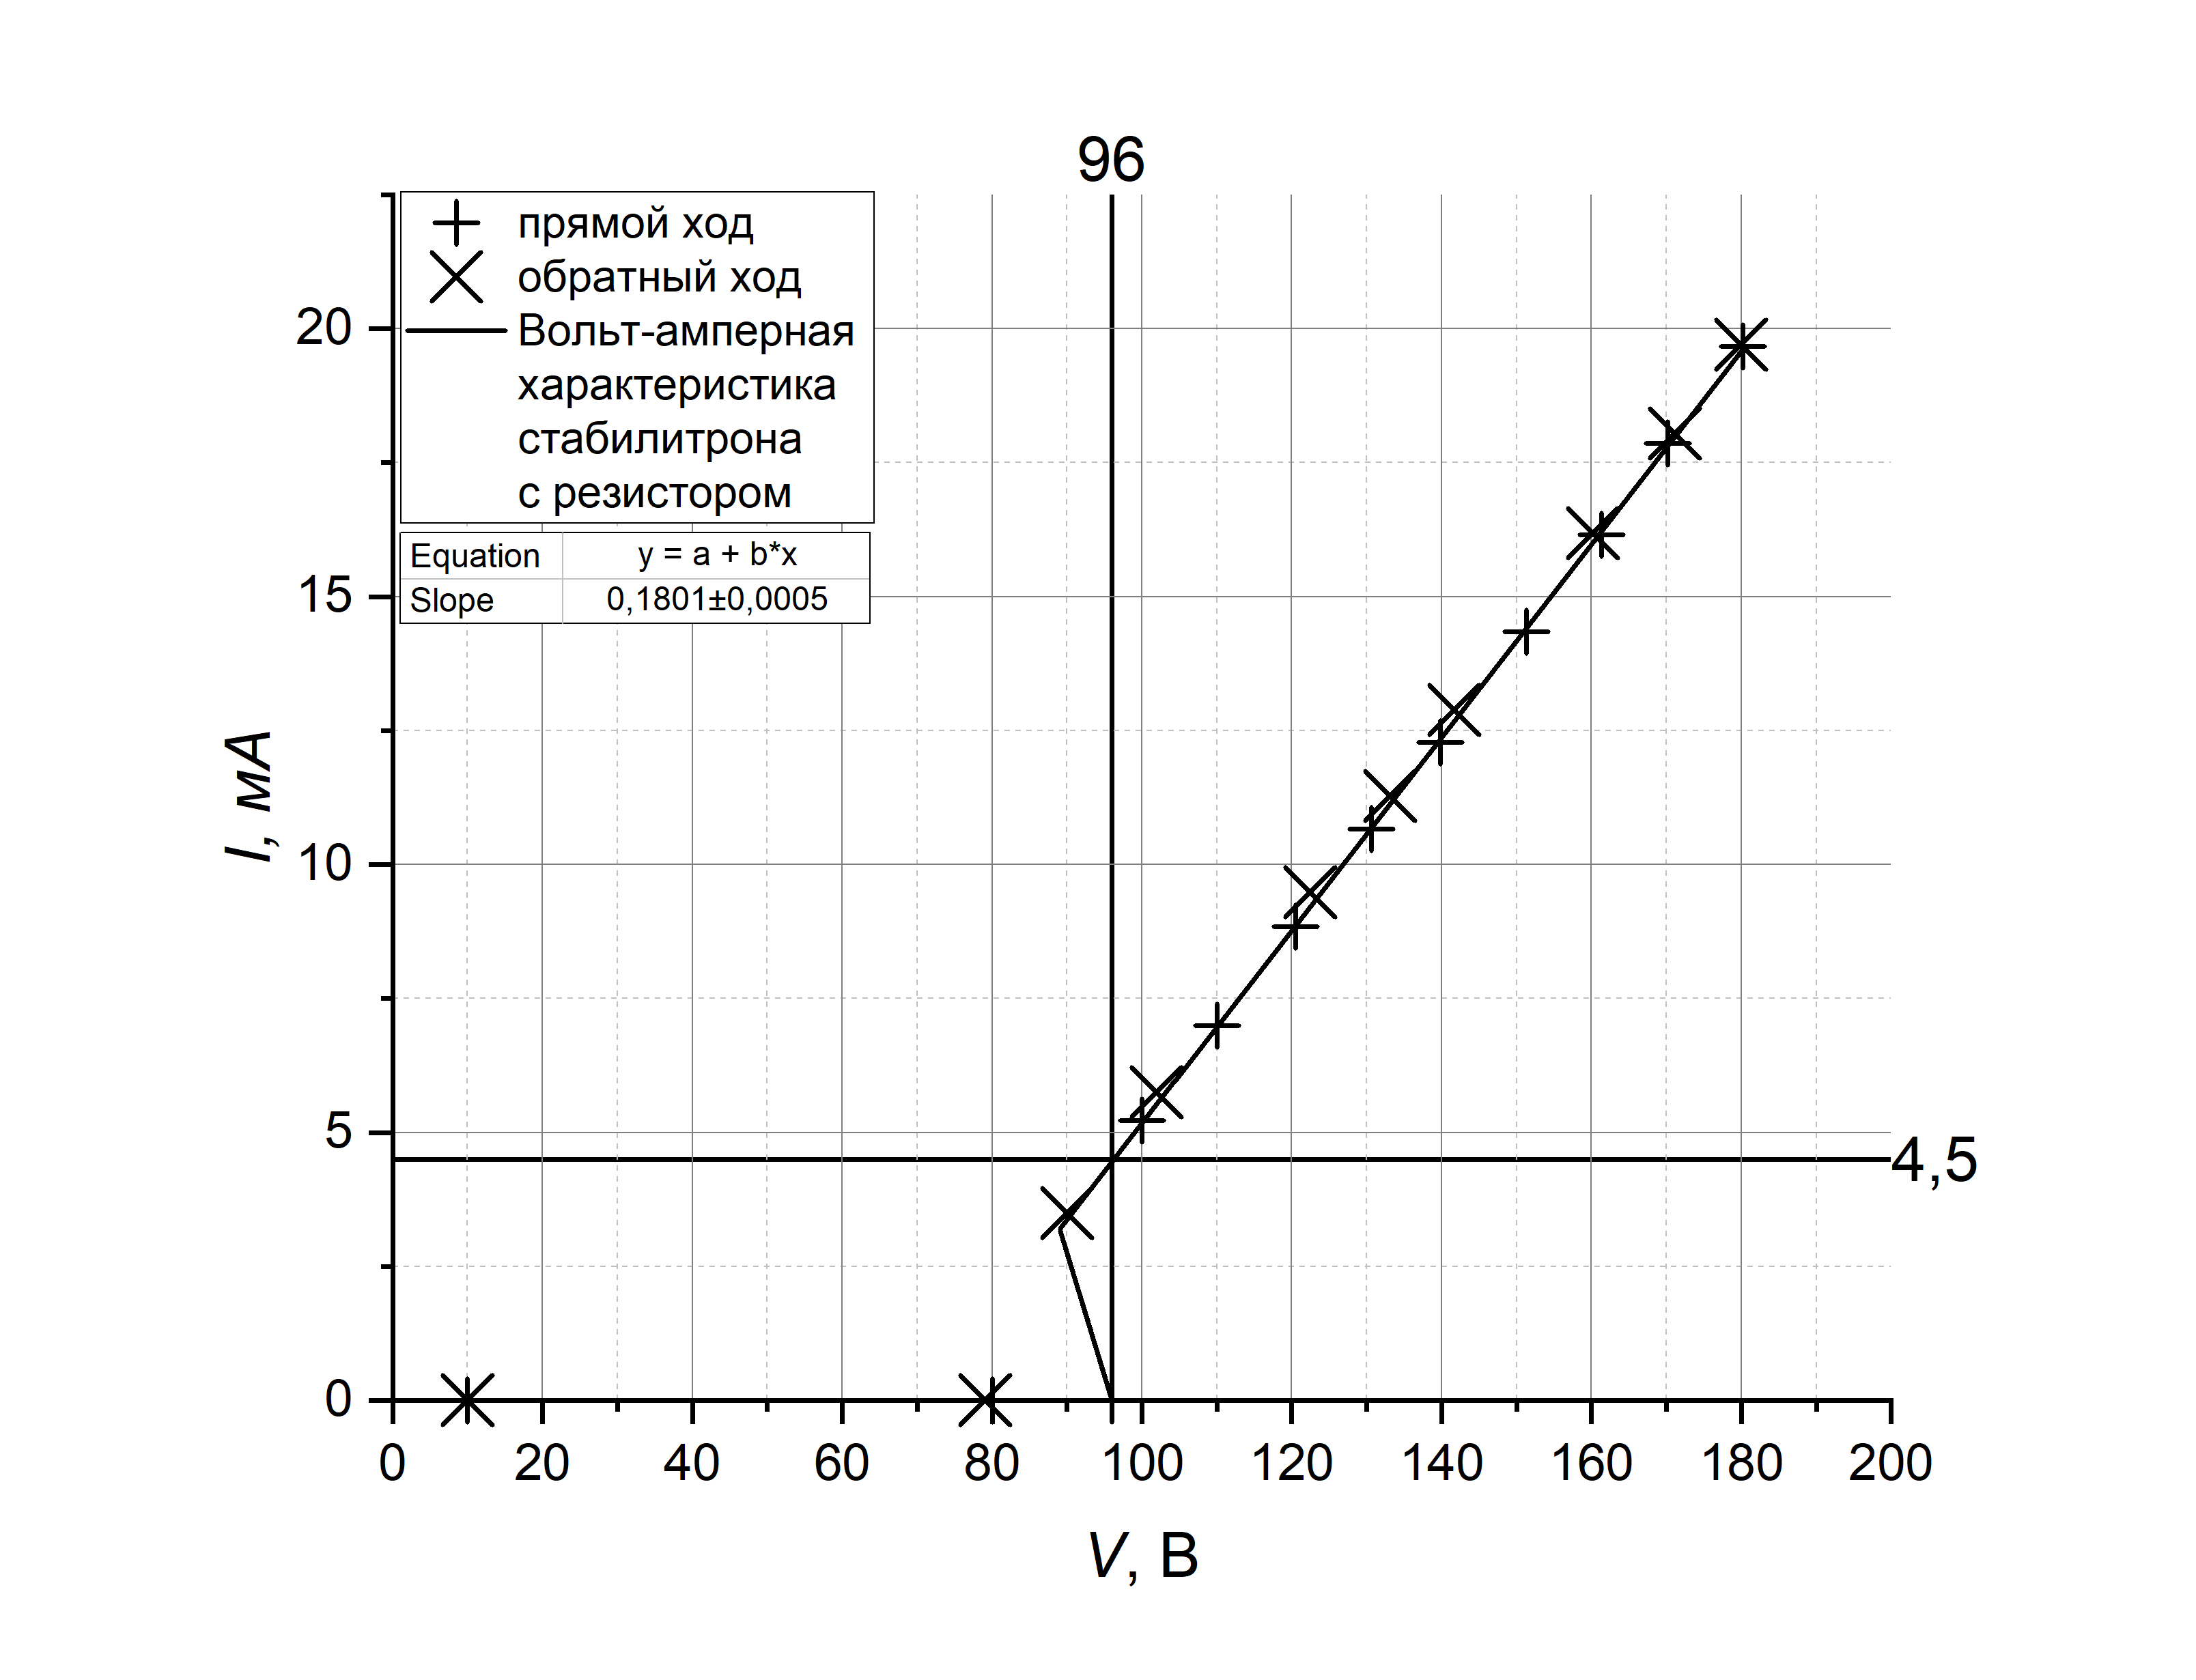
\includegraphics[width = \textwidth]{2.jpg}
Рис. 4: Вольт-амперная характеристика стабилитрона без $r$
\end{center}
\begin{center}
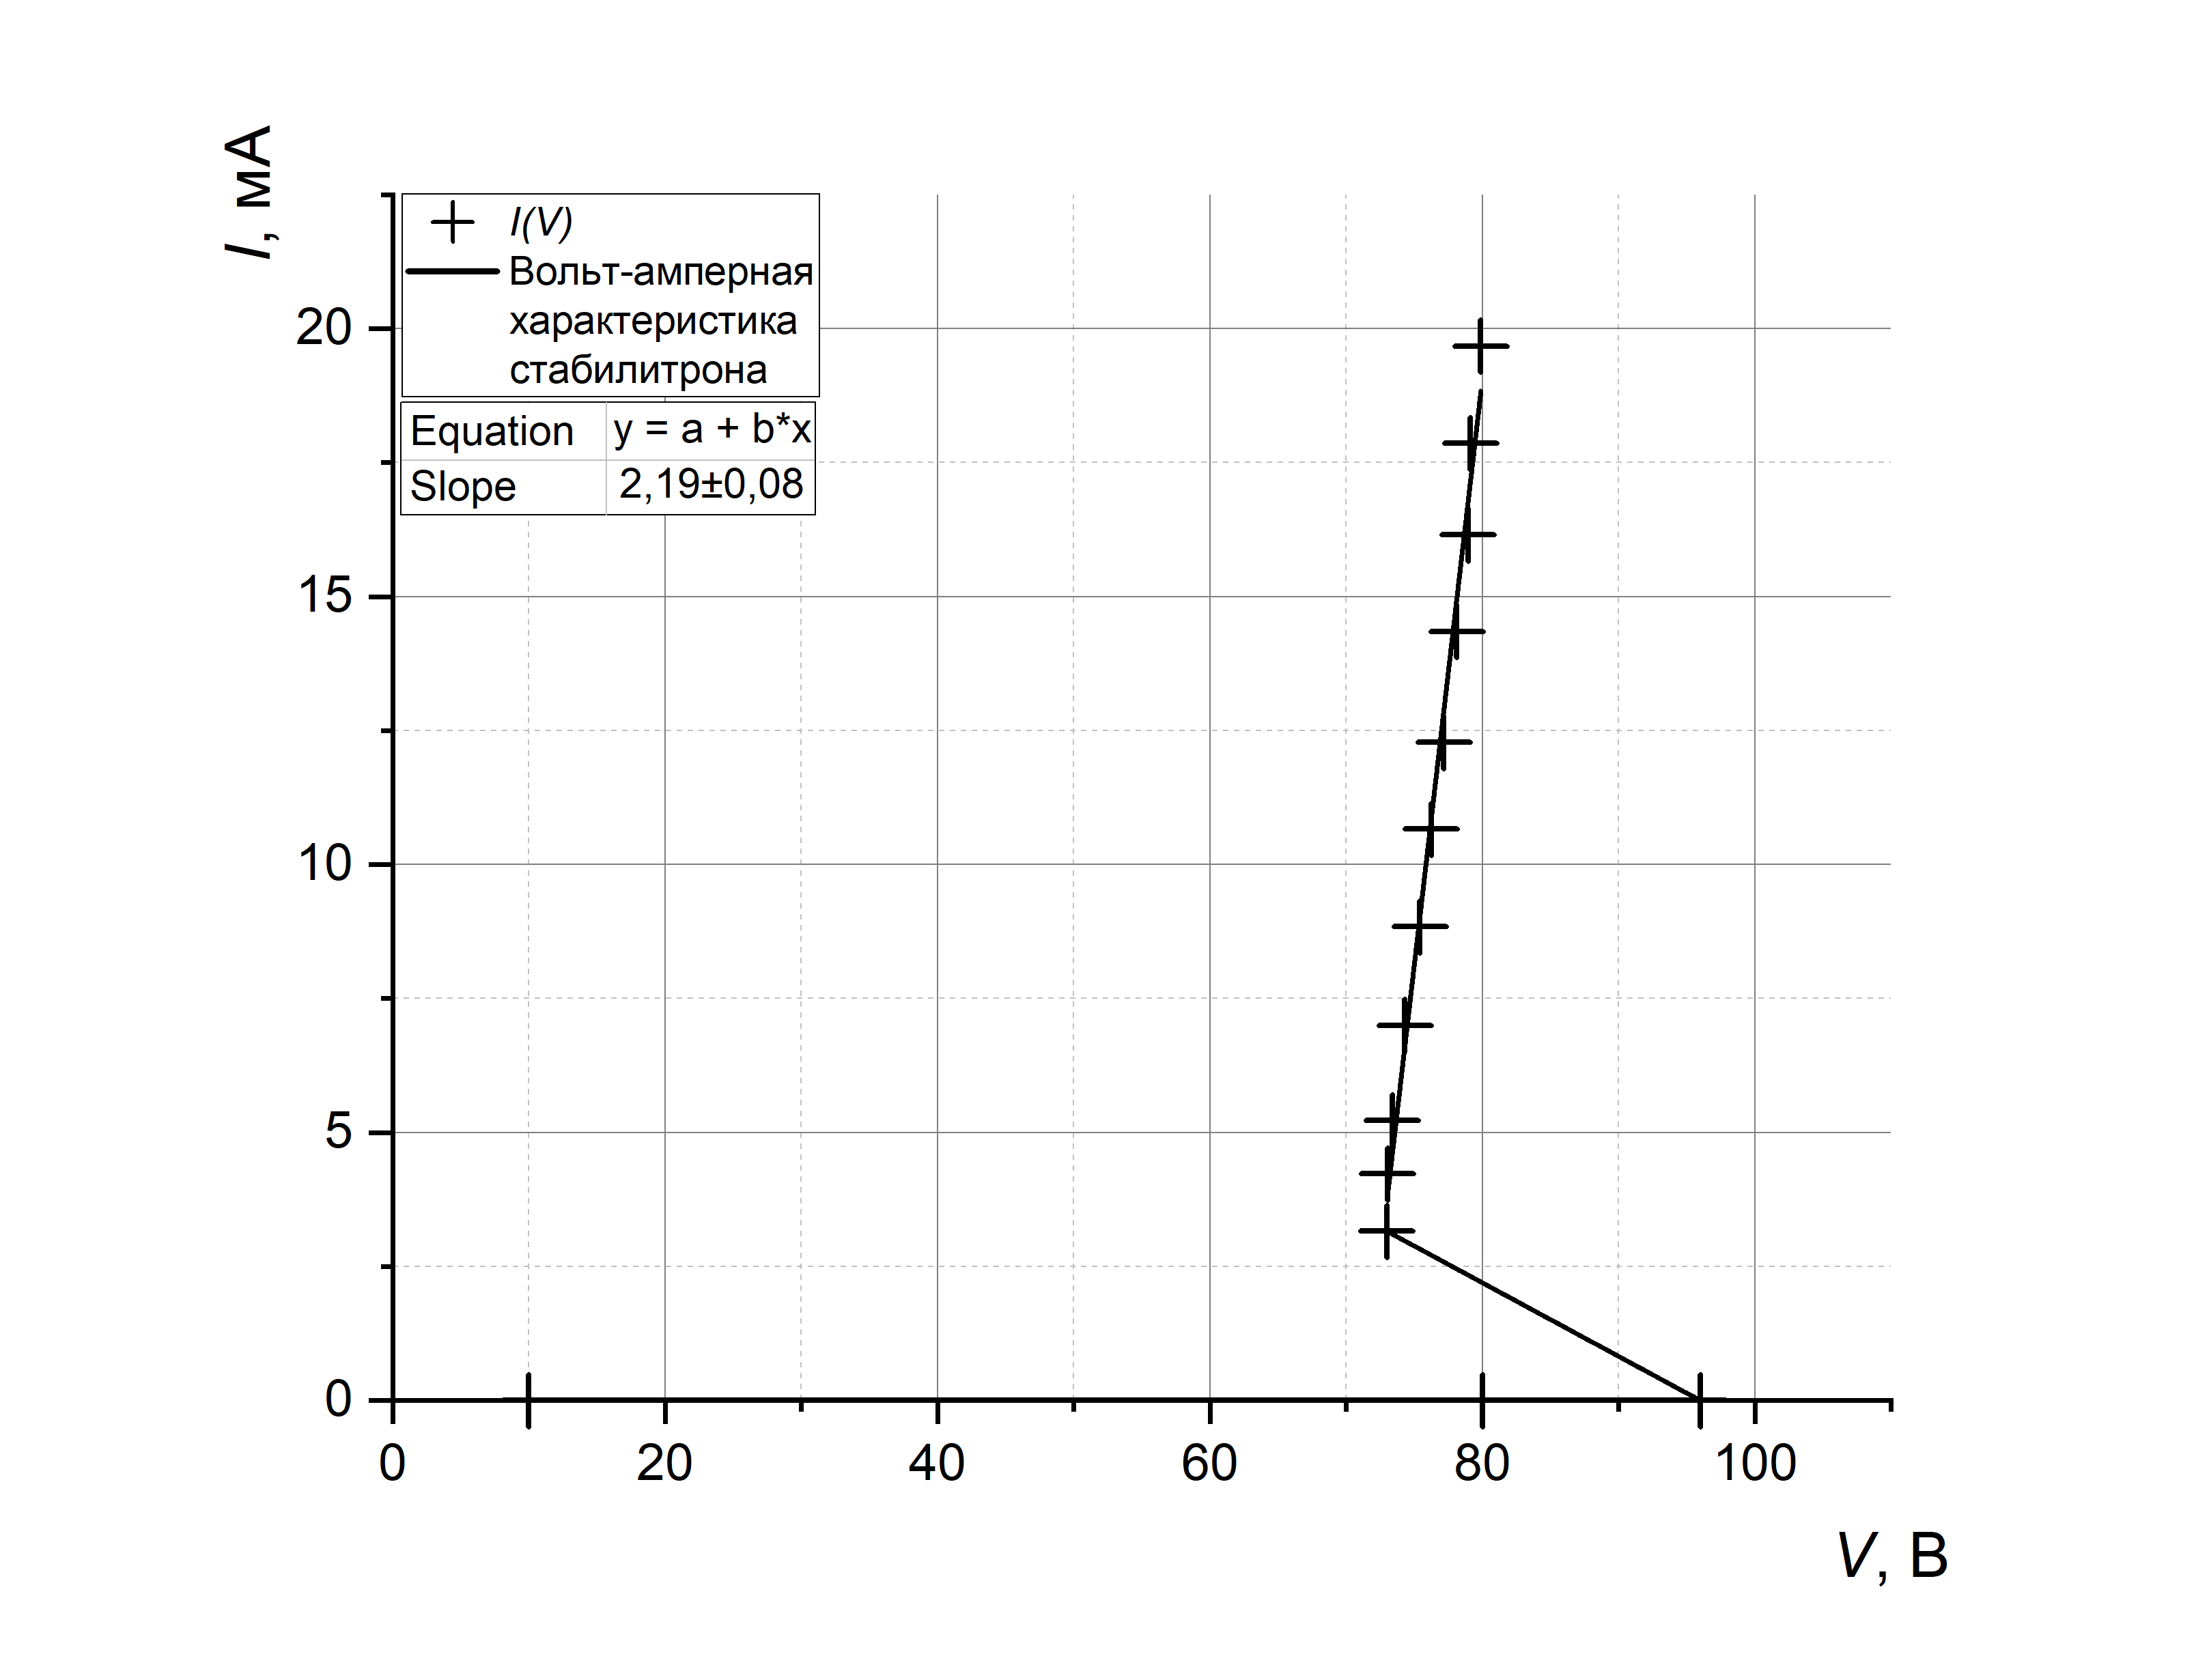
\includegraphics[width = \textwidth]{1.jpg}
Рис. 5: Вольт-амперная характеристика стабилитрона без $r$
\end{center}

В итоге мы получаем, что $V_1 = (96,0 \pm 0,2)$ В, $I_1 = (4,50 \pm 0,02)$ мА, $V_2 = (89,1 \pm 0,2)$ В, $I_2 = (3,16 \pm 0,02)$ мА.
\newpage
\subsection*{Осциллограммы релаксационных колебаний}
В данном разделе мы измеряем зависимость осциллограммы от изменения $R$ и $C$ у установки и сравнения их с теоретическими. 

Сами колебания выглядят следующим образом
\begin{center}
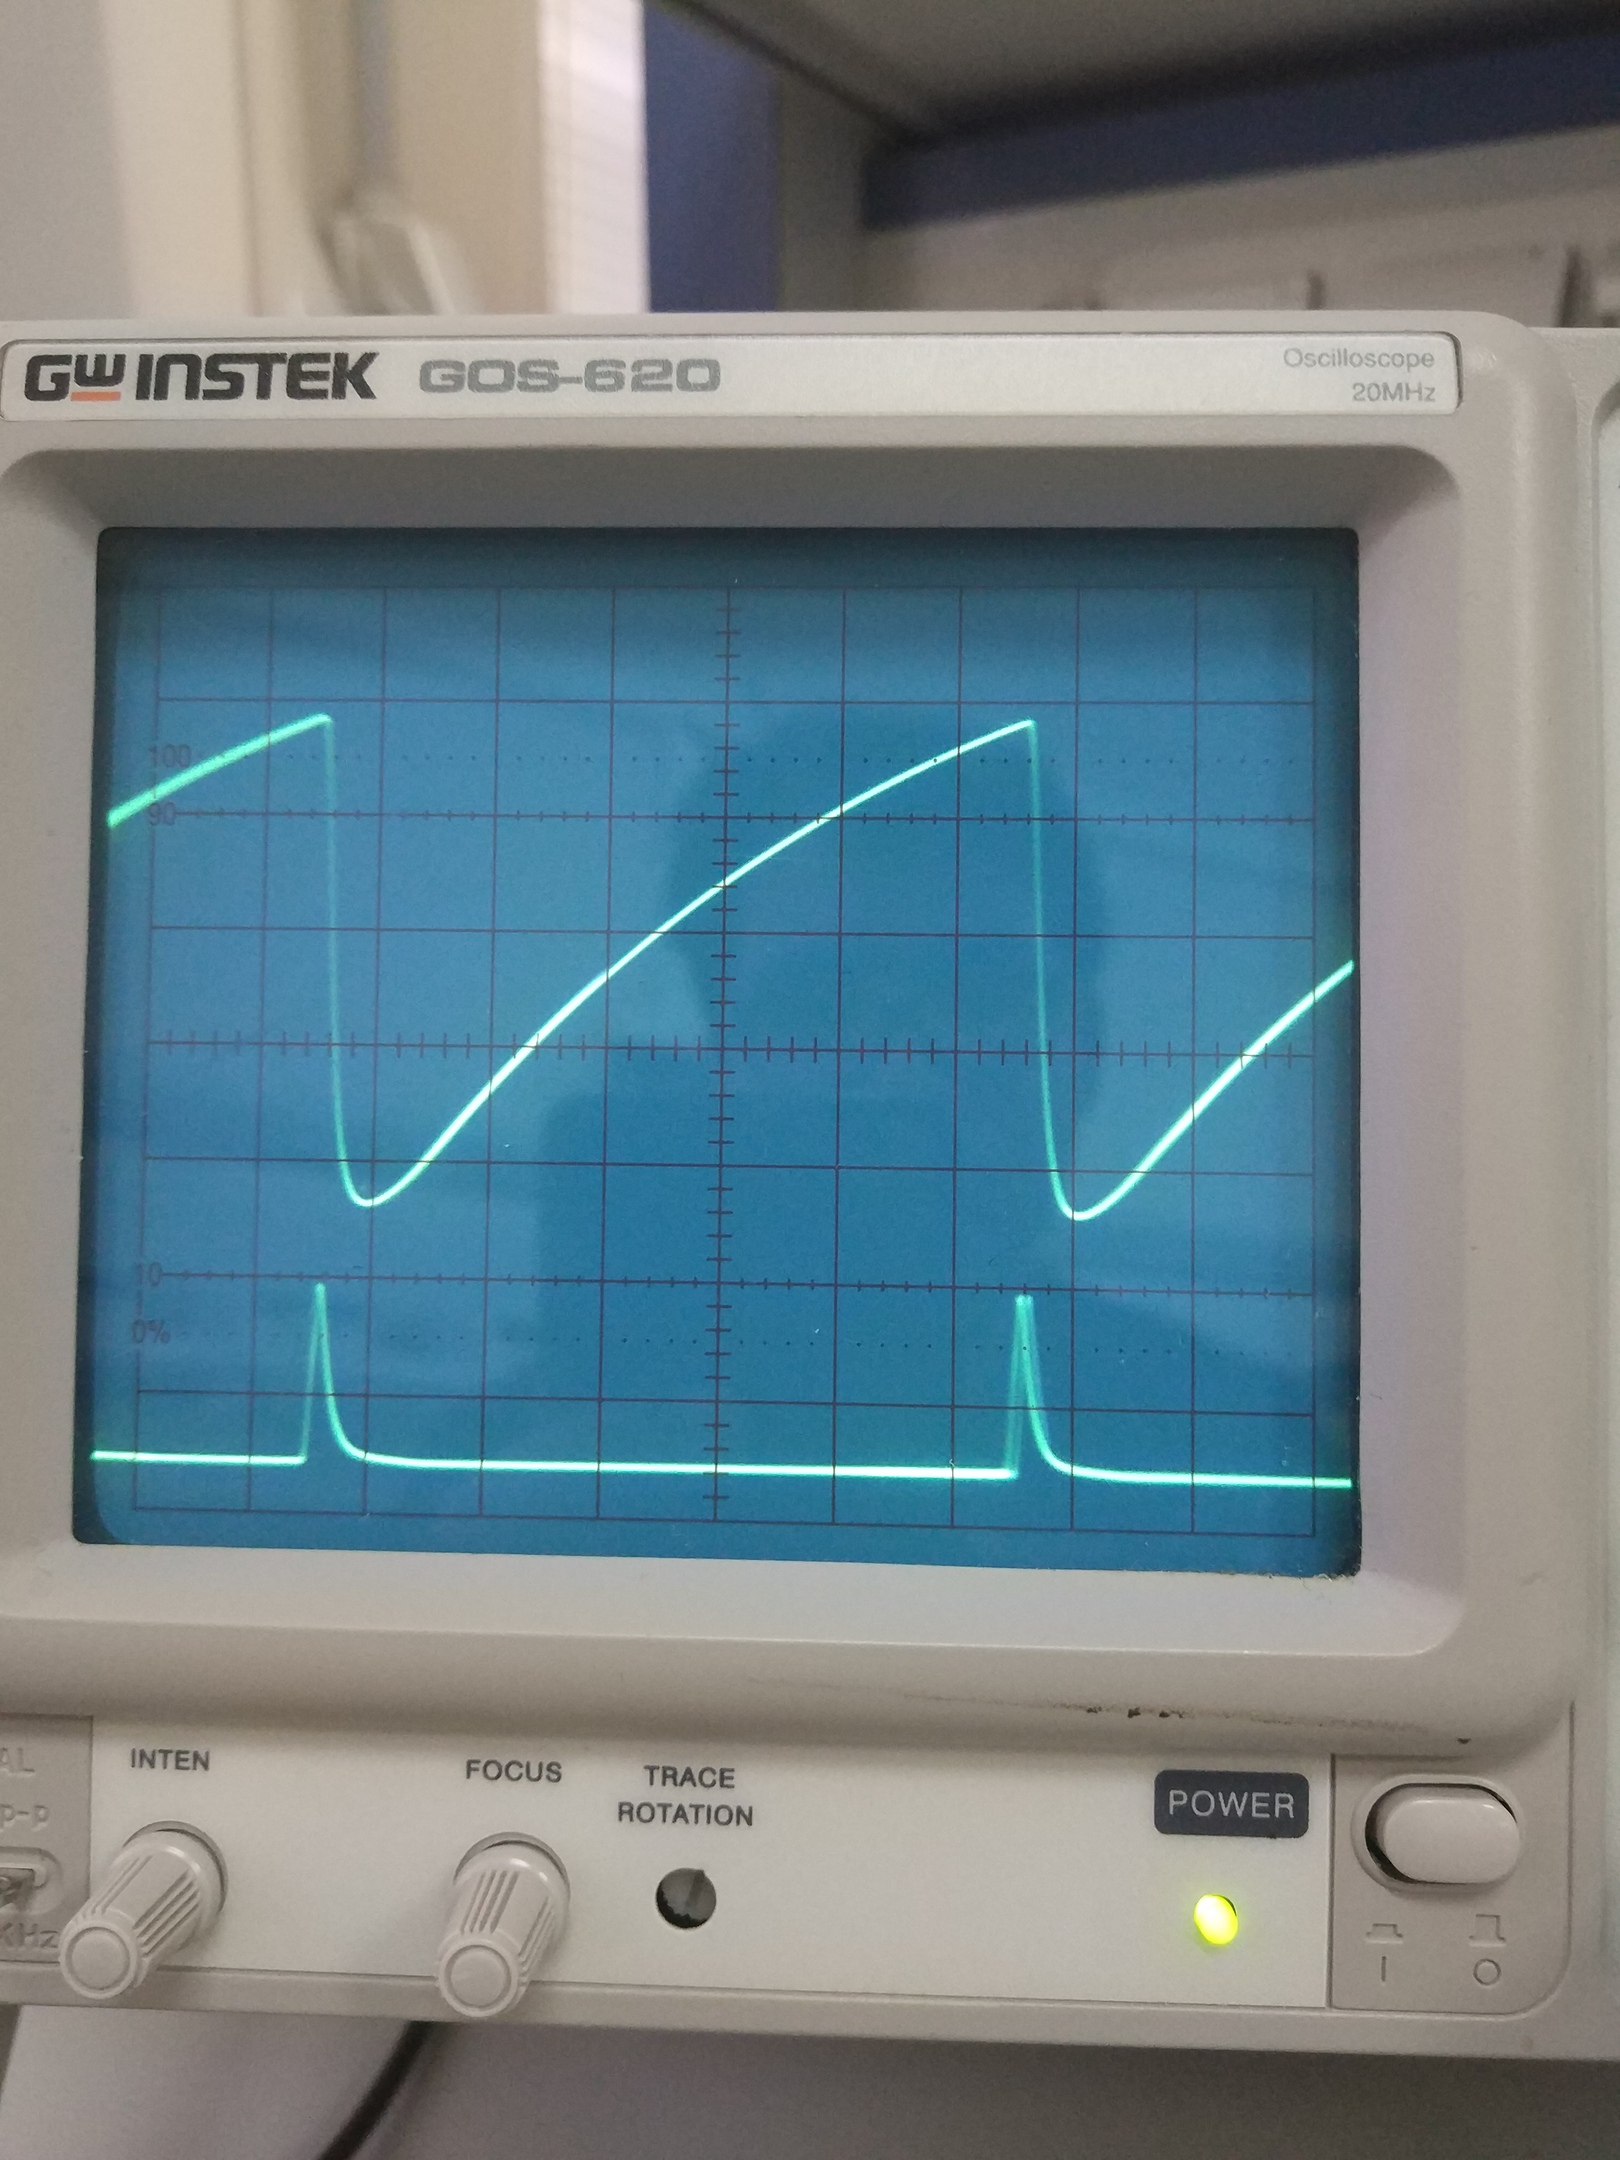
\includegraphics[width = 0.9\textwidth]{7.jpg}
\end{center}

\newpage
Для этого приведем в таблице 2 приведем в параллельных столбцах теоретические и практические значения для данных $R$ и $C$. Так же стоит отметить, что у погрешность измерений периода, сопротивления и емкости составляют $\sigma_T = 0,3$ мс, $\sigma_R = 10$ Ом, $\sigma_C = 2$ нФ. Так же все измерения мы проводим при $U = 132$ В.

\begin{table}[h]
\begin{center}
\begin{tabular}{|c|c|c|c|}
\hline
$C$, нФ & $T$, ед & $T_{exp}$, мс & $T_{theor}$, мс \\ \hline
50      & 6       & 3,0           & 3,0            \\ \hline
45      & 5,4     & 2,7           & 2,7            \\ \hline
40      & 4,8     & 2,4           & 2,4            \\ \hline
35      & 4,2     & 2,1           & 2,1            \\ \hline
30      & 3,6     & 1,8           & 1,8            \\ \hline
25      & 3       & 1,5           & 1,5            \\ \hline
20      & 2,4     & 1,2           & 1,2            \\ \hline
\end{tabular}
\caption{Зависимость $T$ от $C$ при фиксированном $R = 900$ кОм}

\begin{tabular}{|c|c|c|c|}
\hline
$R$, кОм & $T$, ед & $T_{exp}$, мс & $T_{theor}$, мс \\ \hline
900      & 5,8     & 2,9           & 3,0            \\ \hline
800      & 5,2     & 2,6           & 2,7            \\ \hline
700      & 4,6     & 2,3           & 2,3            \\ \hline
600      & 4       & 2,0           & 2,0            \\ \hline
500      & 3,4     & 1,7           & 1,7            \\ \hline
400      & 2,8     & 1,4           & 1,3            \\ \hline
\end{tabular}
\caption{Зависимость $T$ от $R$ при фиксированном $C = 50$ нФ}
\end{center}
\end{table}

По этим таблицам мы видим, что эксперимент сходится с теорией.
\newpage 
\subsection*{Фазовые траектории релаксационных колебаний}
С помощью осциллографа в двухканальном режиме получим изображение фазовой траектории релаксационных колебаний.
\begin{figure}[h]
\begin{center}
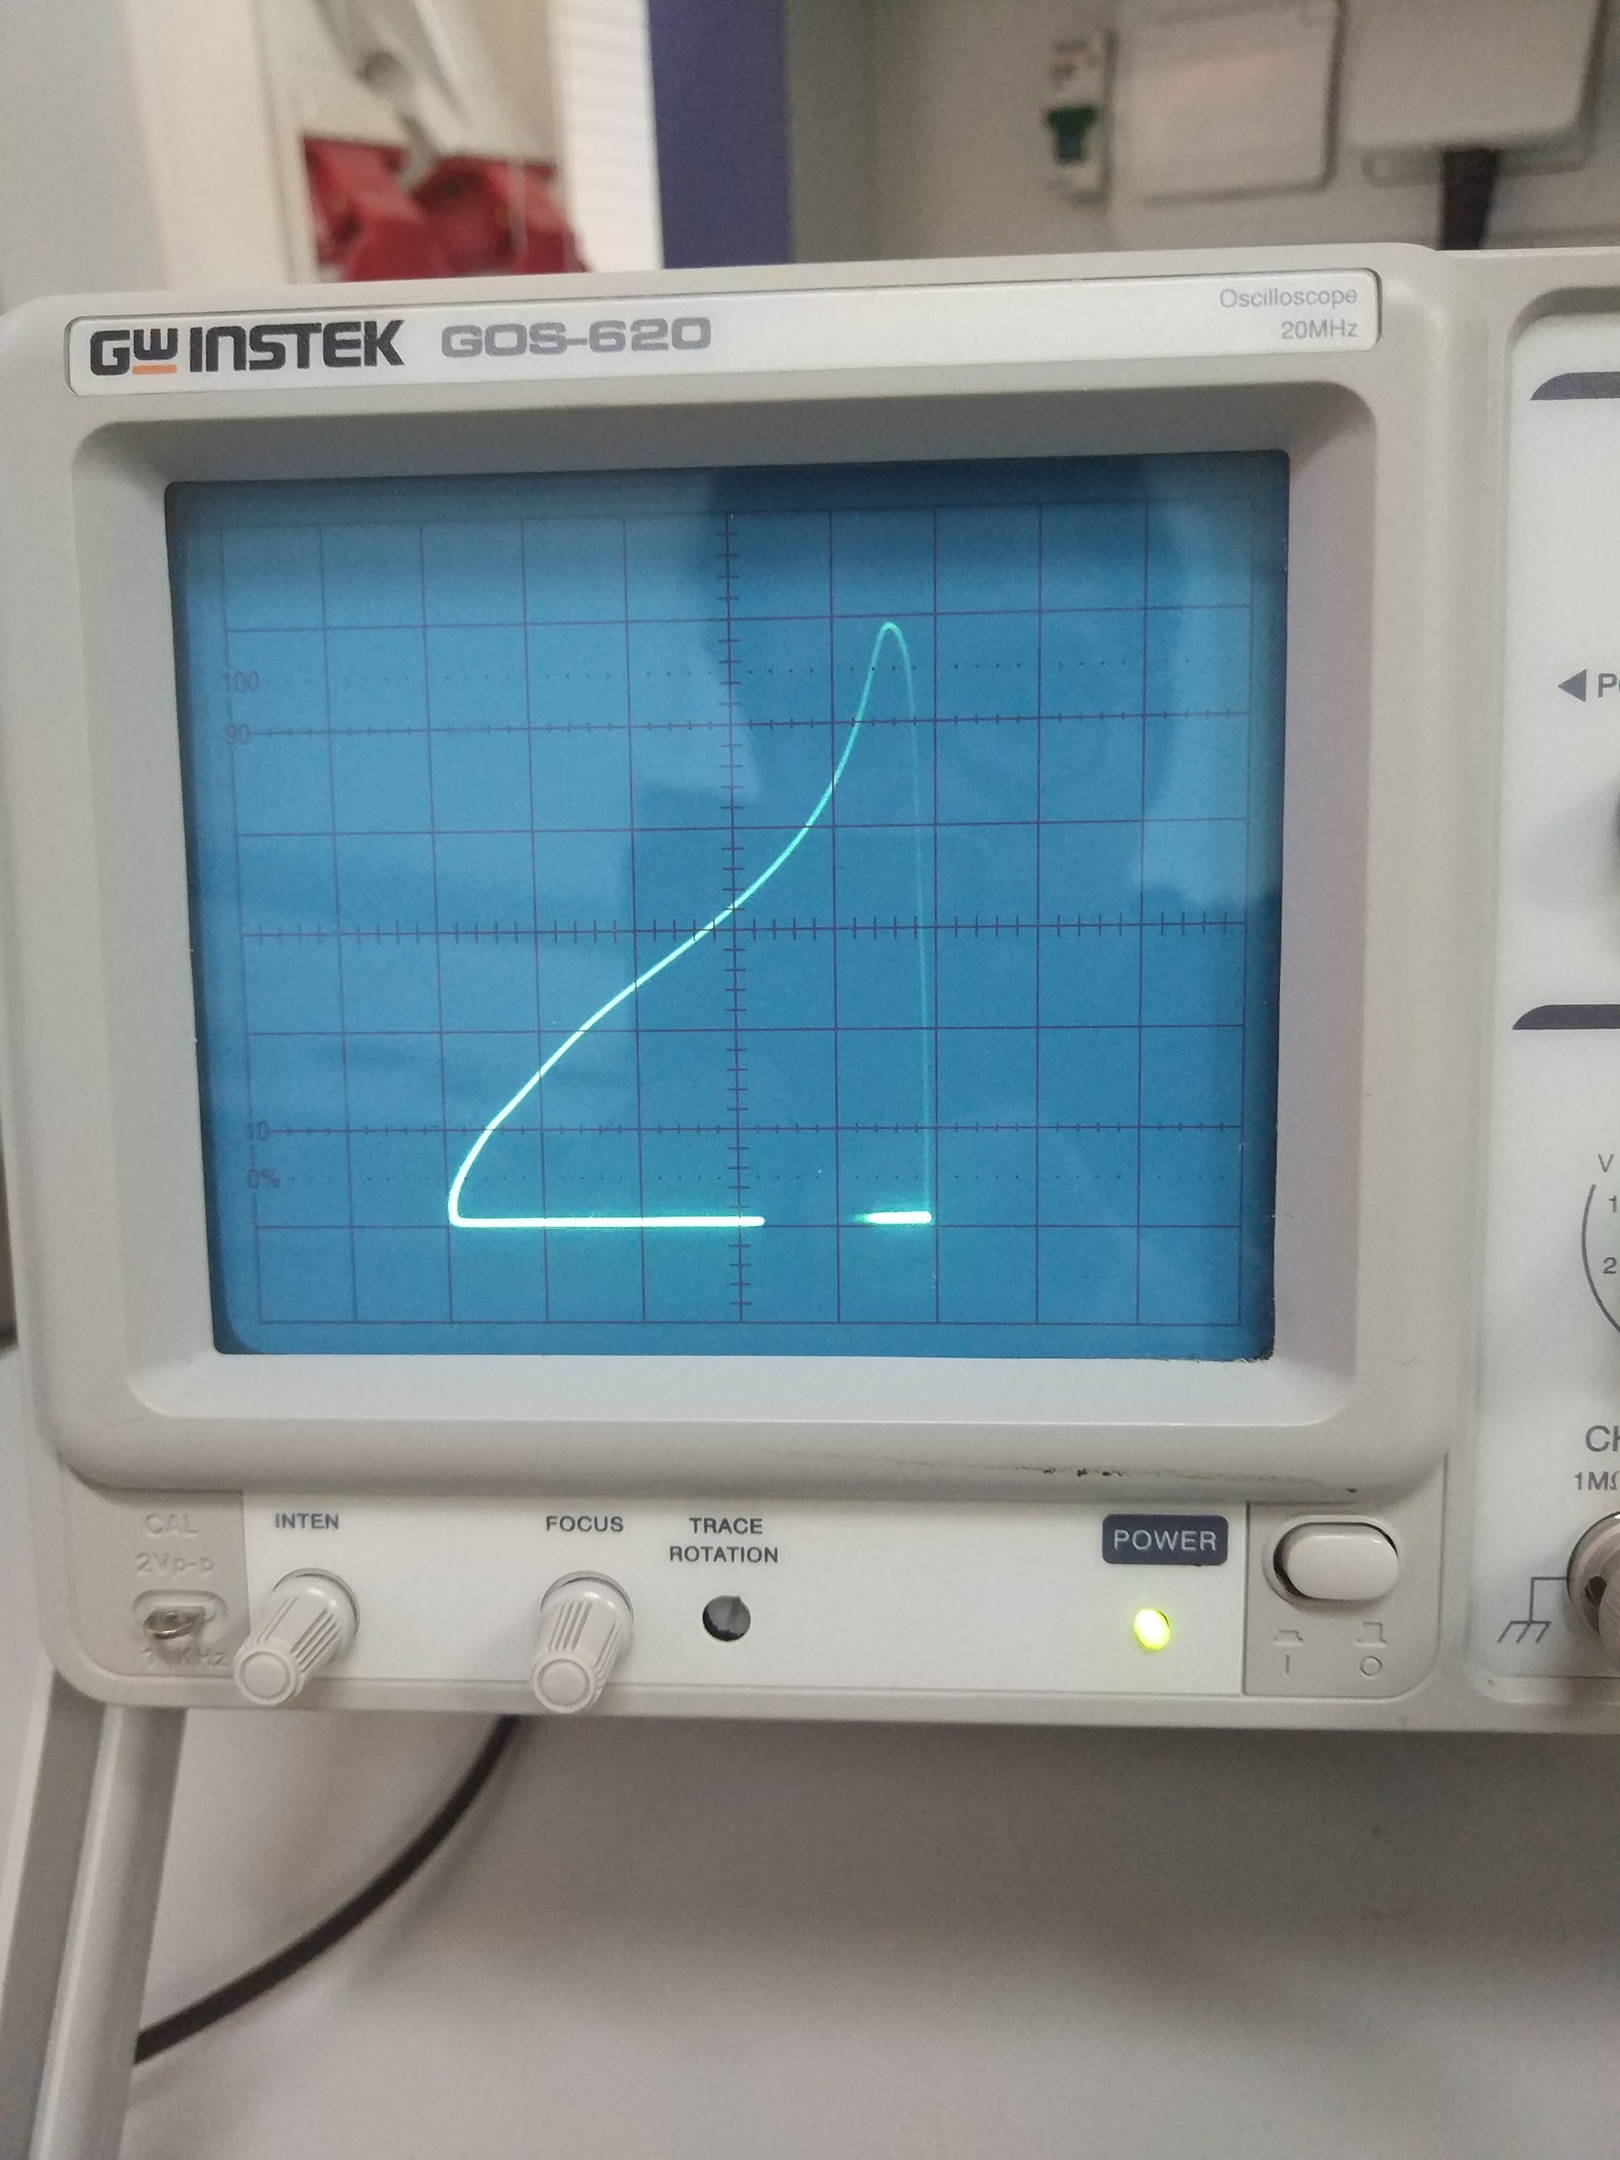
\includegraphics[width = 0.4\textwidth]{6.jpg}
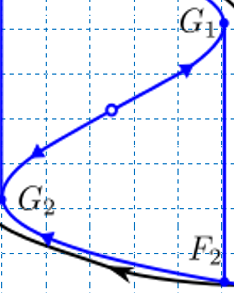
\includegraphics[width = 0.4\textwidth]{9.png}
\caption{Теоретически и практически полученные фазовые кривые}
\end{center}
\end{figure}
И на практике и в теории масштаб такой, что 1 деление по оси $Ox$  --- 2 В, а по оси $Oy$ --- 1 В.
\section*{Вывод}
Мы получили зависимость периода от $R$ и $C$ очень близкие к теоретическим данным, так же мы получили очень похожую на теоретическую вольт-амперную характеристику для стабилитрона. 

Так же в этой лабораторной работе мы изучили релаксационные колебания, но с некоторыми расхождениями от теоретических. Это может быть вызвано тем, что в цепи есть еще дополнительное сопротивление, которое уменьшает напряжение, из-за чего нижняя часть графика в эксперименте вырождается в кривую.
\section*{Литература}
\begin{enumerate}
\item \textbf{Лабораторный практикум по общей физике:} Учебное пособие. В трех томах. Т. 2. Электричество и магнетизм /Гладун А.Д., Александров Д.А., Берулёва Н.С. и др.; Под ред. А.Д. Гладуна - М.: МФТИ, 2007. - 280 с.
\item \textbf{Дополнительное описание лабораторной работы 3.5.3 Вариант 2}: Исследование спектров сигналов; Под ред. МФТИ, 2018 г. - 10 с.
\end{enumerate}
\end{document}